\documentclass[10pt]{beamer}
\usepackage{appendixnumberbeamer}
\usepackage{booktabs}
\usepackage[scale=2]{ccicons}
\usepackage{pgfplots}
\usepackage{xspace}
\usepackage{xcolor}
\usepackage{xurl}
\usepackage{caption}
\usepackage{soul}

\DeclareMathOperator*{\argmax}{argmax} 
\newtheorem{axiom}{Axiom} 

\usetheme[progressbar=frametitle]{metropolis}
\usepgfplotslibrary{dateplot}
\newcommand{\themename}{\textbf{\textsc{metropolis}}\xspace}
\captionsetup[figure]{labelformat=empty}

% ---------------------------------------------------------
\title{A way around the\\exploration-exploitation dilemma}
\date{}
\author{Erik J Peterson}
\institute{Research fellow | CoAxLab\\
Carnegie Mellon University\\
\url{robotpuggle.com}}

% ---------------------------------------------------------
\begin{document}
\maketitle

% \begin{frame}{Table of contents.}
%   \setbeamertemplate{section in toc}[sections numbered]
%   \tableofcontents%[hideallsubsections]
% \end{frame}

% ---------------------------------------------------------
% \begin{frame}[fragile]{Astrocytes and cognition!?}
% \begin{itemize}
%     \item Classically astrocytes have been considered neural support cells.
%     \item Growing evidence that astrocytes can directly drive cognition and motor behavior.
    

% \end{itemize}
% \end{frame}
\begin{frame}[fragile]{The dilemma.}
\begin{figure}
    \centering
    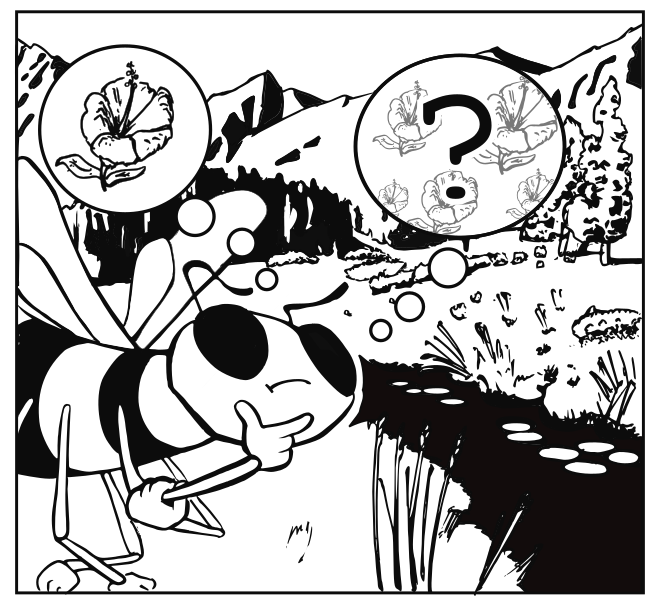
\includegraphics[scale=0.8]{images/left_bee.png} 
    \caption{Should I exploit an available reward, or explore to try and find more rewards?}
\end{figure}
\end{frame}

\begin{frame}[fragile]{The dilemma.}
\begin{columns}
\column{0.5\textwidth}
\centering
\begin{itemize}
    \item Exploration is the problem.
\end{itemize}

\column{0.5\textwidth}
\centering
\begin{figure}
    \centering
    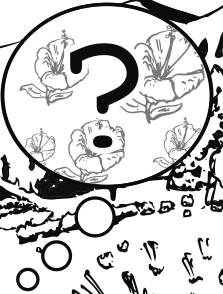
\includegraphics[scale=1.5]{images/bee_explore.png} 
    \caption{}
\end{figure}
\end{columns}
\end{frame}

\begin{frame}[fragile]{The dilemma.}
\begin{columns}
\column{0.5\textwidth}
\centering
\begin{itemize}
    \item Exploration is an intractable problem.
    \begin{itemize}
    \item There is no optimal solution.
    \item Only average solutions. \cite{Thrun1992a,Dayan1996,Findling2018,Gershman2018b}.
    \end{itemize}
\end{itemize}

\column{0.5\textwidth}
\centering
\begin{figure}
    \centering
    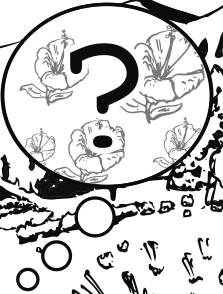
\includegraphics[scale=1.5]{images/bee_explore.png} 
    \caption{}
\end{figure}
\end{columns}
\end{frame}

\begin{frame}[fragile]{The dilemma.}
\begin{columns}
\column{0.5\textwidth}
\centering
\begin{itemize}
    \item An average life is full of regret.
\end{itemize}

\column{0.5\textwidth}
\centering
\begin{figure}
    \centering
    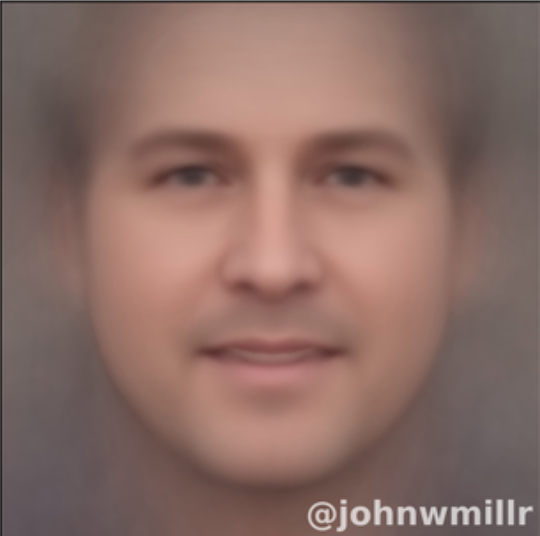
\includegraphics[scale=0.4]{images/average_country_singer.png} 
    \caption{\footnotesize{The average country singer.}}
\end{figure}
\end{columns}
\end{frame}

\begin{frame}[fragile]{The dilemma.}
\begin{itemize}
    \item An average life is full of regret, $G$.
    \item Where $G = V^* - V_a$
\end{itemize}
\end{frame}

\begin{frame}[fragile]{Our goal.}
\begin{itemize}
    \item To lead a life of no regret.
\end{itemize}
\end{frame}

\begin{frame}[fragile]{Our goal.}
\begin{itemize}
    \item To lead a life of no regret, $G=0$
    \item ...for all $s \in S$, $a \in A$ and $t \leq T$.
\end{itemize}
\end{frame}

\begin{frame}[fragile]{Why do animals explore?}
\begin{itemize}
    \item Find rewards
    \item 
    \item
\end{itemize}
\end{frame}

\begin{frame}[fragile]{Why do animals explore?}
\begin{itemize}
    \item \st{Find rewards}
    \item 
    \item
\end{itemize}
\end{frame}

\begin{frame}[fragile]{Why do animals explore?}
\begin{itemize}
    \item \st{Find rewards}
    \item Learn about their niche
    \item Learn about other animals
\end{itemize}
\end{frame}

\begin{frame}[fragile]{Why do animals explore?}
\begin{columns}
\column{0.5\textwidth}
\centering
\begin{itemize}
    \item \st{Find rewards}
    \item They are curious
\end{itemize}

\column{0.5\textwidth}
\begin{figure}
    \centering
    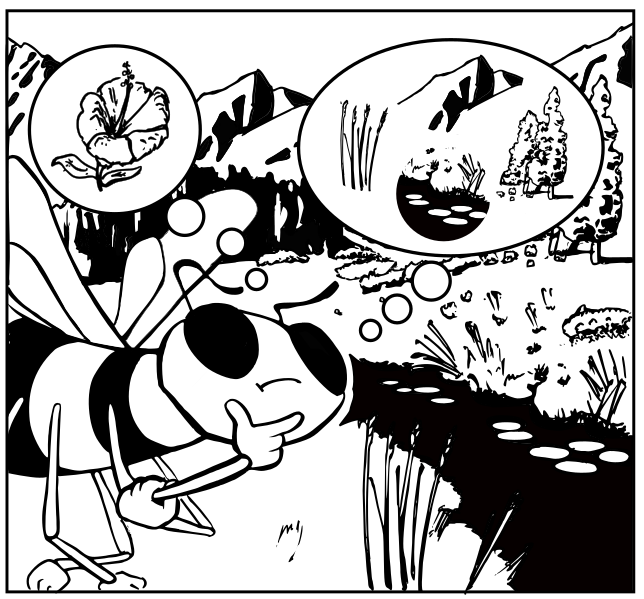
\includegraphics[scale=0.8]{images/right_bee.png}
    \caption{}
\end{figure}
\end{columns}
\end{frame}

\begin{frame}[fragile]{Curiosity is not a luxury.}
\begin{itemize}
    \item If you do not learn about your niche, you die.
\end{itemize}
\end{frame}

\begin{frame}[fragile]{Big conjecture \#1.}
\begin{center}
    Information is fundamentally valuable.
\end{center}
\end{frame}

\begin{frame}[fragile]{Big conjecture \#2.}
\begin{center}
    Exploration for reward is never needed. The only exploratory behavior an animal needs is that which builds its world model.
\end{center}
\end{frame}

\begin{frame}[fragile]{\textit{Ad hoc} curiosity.}
\begin{itemize}
    \item Novelty
    \item Counts/Successors
    \item Information gain
    \item Entropy
    \item State prediction
\end{itemize}
\end{frame}

\begin{frame}[fragile]{Reinforcement learning}
\begin{itemize}
    \item Reward learning has made progress because it has a clear objective:
    \begin{itemize}
        \item $ \max \sum_T R$
    \end{itemize}
\end{itemize}
\end{frame}

\begin{frame}[fragile]{Goal.}
\begin{itemize}
    \item Curiosity learning needs a clear and common objective:
    \begin{itemize}
        \item $ \max \sum_T E$
    \end{itemize}
\end{itemize}
\end{frame}

\begin{frame}[fragile]{What is \textit{E}?}
\begin{itemize}
    \item Novelty?
    \item Counts/Successors?
    \item Information gain?
    \item Mutual information? 
    \item State prediction?
\end{itemize}
\end{frame}

\begin{frame}[fragile]{What is \textit{E}?}
\begin{itemize}
    \item Novelty?
    \item Counts/Successors?
    \item Information gain?
    \item Mutual information?
    \item State prediction?
    \item \alert{Free energy?}
\end{itemize}
\end{frame}

\begin{frame}[fragile]{A minimum definition.}
\begin{itemize}
    \item At an \textit{absolute minimum} what do we need to value information ?
\end{itemize}
\end{frame}

\begin{frame}[fragile]{A minimum definition.}
\textit{What do we need to value information?}
\begin{enumerate}
    \item A world
    % \item Actions
    % \item A memory
\end{enumerate}
\end{frame}

\begin{frame}[fragile]{A minimum definition.}
\textit{What do we need to value information?}
\begin{enumerate}
    \item A world
    \item Actions
    % \item A memory
\end{enumerate}
\end{frame}

\begin{frame}[fragile]{A minimum definition.}
\textit{What do we need to value information?}
\begin{enumerate}
    \item A world
    \item Actions
    \item A memory
\end{enumerate}
\end{frame}

\begin{frame}[fragile]{A minimum definition.}
\textit{What do we need to value information?}
\begin{enumerate}
    \item A world
    \item Actions
    \item A memory $\Leftrightarrow$ \textit{world model}
\end{enumerate}
\end{frame}

\begin{frame}[fragile]{A minimum definition.}
\textit{What do we need to value information?}
\begin{enumerate}
    \item A world, $S^n$
    \item Actions $A^m$
    \item A memory, $M^k$
\end{enumerate}
\end{frame}

\begin{frame}[fragile]{A minimum memory.}
\textit{What does a memory need to be a memory?}
\begin{enumerate}
    \item Finite
    % \item It must remember
    % \item It must recall
    % \item It must forget
\end{enumerate}
\end{frame}

\begin{frame}[fragile]{A minimum memory.}
\textit{What does a memory need to be a memory?}
\begin{enumerate}
    \item Finite
    \item It must remember
    % \item It must recall
    % \item It must forget
\end{enumerate}
\end{frame}

\begin{frame}[fragile]{A minimum memory.}
\textit{What does a memory need to be a memory?}
\begin{enumerate}
    \item Finite
    \item It must remember
    \item It must recall
    % \item It must forget
\end{enumerate}
\end{frame}

\begin{frame}[fragile]{A minimum memory.}
\textit{What does a memory need to be a memory?}
\begin{enumerate}
    \item Finite
    \item It must remember
    \item It must recall
    \item It must forget
\end{enumerate}
\end{frame}

\begin{frame}[fragile]{A minimum memory.}
\textit{What does a memory need to be a memory?}
\begin{enumerate}
    \item Finite, $M^k$
    \item It must remember, $f : s, M \rightarrow M'$ where $s \in S$
    \item It must recall, $g : s, M \rightarrow \hat s$
    \item It must forget, $f^{-1} : s, M' \rightarrow M$
\end{enumerate}
\end{frame}

\begin{frame}[fragile]{A minimum memory.}
\textit{What does a memory need to be a memory?}
\begin{enumerate}
    \item Finite, $M^k$
    \item It must remember, $f : s, M \rightarrow M'$ where $s \in S$
    \item It must recall, $g : s, M \rightarrow \hat s$
    \item It must forget, $f^{-1} : s, M' \rightarrow M$
    \item Made of real numbers, $M \in \mathbb{R}$
\end{enumerate}
\end{frame}

\begin{frame}[fragile]{Commonalities?}
\begin{itemize}
    \begin{itemize}
    \item Novelty
    \item Counts/Successors
    \item Information gain
    \item Mutual information
    \item State prediction
    \end{itemize} \\
    \item \textbf{Value comes from how memory changes?}
\end{itemize}
\end{frame}

\begin{frame}[fragile]{Axiom 1.}
\begin{axiom}
    [Axiom of Change] The value of information $E$ depends only on the total distance $M$ moves by making observation $s$.
    \label{ax:1} 
\end{axiom}
\end{frame}

\begin{frame}[fragile]{Minimal distance $d$.}
\begin{itemize}
    \item Let $\delta = d(m,m')$, where $m \in M$ and $m' \in M'$
    \item $\delta \ge 0$
    \item $\sum \delta = 0$ only if $M = M'$
    \item ($d$ is a pre-metric)
\end{itemize}
\end{frame}

% \begin{frame}[fragile]{Minimal distance $d$.}
% \begin{itemize}
%     \item Let $\delta = d(m,m')$, where $m \in M$ and $m' \in M'$
%     \item $\delta \ge 0$
%     \item $\sum \delta = 0$ only if $M = M'$
%     \item \alert{$d$ is a pre-metric}
% \end{itemize}
% \end{frame}

% \begin{frame}[fragile]{Minimal distance $d$.}
% \begin{itemize}
%     \item Let $\delta = d(m,m')$, where $m \in M$ and $m' \in M'$
%     \item $\delta \ge 0$
%     \item $\sum \delta = 0$ only if $M = M'$
%     \item \textit{Optional}: 
%     \begin{itemize}
%         \item $d(m,m') = d(m',m)$ 
%         \item triangle inequality
%     \end{itemize}
% \end{itemize}
% \end{frame}

\begin{frame}[fragile]{Total distance $||\Delta||$.}
\begin{itemize}
\item The total distance is the norm of $\Delta$, $||\Delta||$
\item Where $\Delta = \{\delta_1, \delta_2,...,\delta_K\}$
% \item \textbf{Let $E \equiv ||\Delta||$}
\end{itemize}
\end{frame}

\begin{frame}[fragile]{Total distance $||\Delta||$.}
\begin{itemize}
\item The total distance is the norm of $\Delta$, $||\Delta||$
\item Where $\Delta = \{\delta_1, \delta_2,...,\delta_K\}$
\item \textbf{Let $E \equiv ||\Delta||$}
\end{itemize}
\end{frame}

\begin{frame}[fragile]{What is $E$.}
\textbf{Axiom 1 $\rightarrow ||\Delta||$.}
\end{frame}

\begin{frame}[fragile]{Examples.}
\textit{Choose $\{M, f, g, d\}$}.
\begin{itemize}
    \item 
\end{itemize}
\end{frame}

\begin{frame}[fragile]{Examples.}
\textit{Choose $\{M, f, g, d\}$}.
\begin{itemize}
    \item A novelty world model:
    \begin{itemize}
        \item $M \in \mathbb{R}^n$
        \item $f,g: $ add $s$, returns $1$ if no $s$ 
        \item $d: |m - m'|^1$ (the \textit{l1 norm} or \textit{Manhattan distance})
    \end{itemize}
\end{itemize}
\end{frame}

\begin{frame}[fragile]{Examples.}
\textit{Choose $\{M, f, g, d\}$}.
\begin{itemize}
    \item A count-based world model:
    \begin{itemize}
        \item $M \in \mathbb{Z}^n$
        \item $f,g: $ counts $s$, returns counts of $s$
        \item $d: |m - m'|^1$ 
    \end{itemize}
\end{itemize}
\end{frame}

\begin{frame}[fragile]{Examples.}
\textit{Choose $\{M, f, g, d\}$}.
\begin{itemize}
    \item A compressed world model:
    \begin{itemize}
        \item $W^c < \mathbb{R}^n$
        \item $f,g: $ lossy encoder, returns $\hat s$
        \item $d: \sqrt{|w - w'|^2}$ euclidean distance on weight parameters, $W$
    \end{itemize}
\end{itemize}
\end{frame}

\begin{frame}[fragile]{Examples.}
\textit{Choose $\{M, f, g, d\}$}.
\begin{itemize}
    \item A compressed world model:
    \begin{itemize}
        \item Linear regression (regularized)
        \item GAN
        \item VAE
    \end{itemize}
\end{itemize}
\end{frame}

\begin{frame}[fragile]{Examples.}
\textit{Choose $\{M, f, g, d\}$}.
\begin{itemize}
    \item An episodic world model:
    \begin{itemize}
        \item $M \in \mathbb{R}^n$
        \item $f,g: $ store $s$, recall $s$
        \item $d: \sqrt{|m - m'|^2}$ 
    \end{itemize}
\end{itemize}
\end{frame}

\begin{frame}[fragile]{Examples.}
\textit{Choose $\{M, f, g, d\}$}.
\begin{itemize}
    \item An categorization world model:
    \begin{itemize}
        \item $W^c \leq \mathbb{R}^n$
        \item $f,g: $ categorize $s$, recall category of $s$
        \item $d: |m - m'|^1$ or 
        \item $d: \sqrt{|w - w'|^2}$ euclidean distance on weight parameters, $W$
    \end{itemize}
\end{itemize}
\end{frame}

\begin{frame}[fragile]{Examples.}
\textit{Choose $\{M, f, g, d\}$}.
\begin{itemize}
    \item An categorization world model:
    \begin{itemize}
        \item Clustering (\textit{e.g.}, K-means)
        \item Classification (\textit{e.g.}, SVM, Random Forrest)
    \end{itemize}
\end{itemize}
\end{frame}

\begin{frame}[fragile]{Examples.}
\textit{Choose $\{M, f, g, d\}$}.
\begin{itemize}
    \item A Bayesian world model:
    \begin{itemize}
        \item $M \in \mathbb{R}^{nm}$
        \item $f,g: $ Bayes rule
        \item $d \approx KL-divergence$
    \end{itemize}
\end{itemize}
\end{frame}

\begin{frame}[fragile]{Axiom 2.}
\begin{axiom}
	[Axiom of Equilibrium] To be valuable an observation $s$ must be learnable by $M$. 
\label{ax:5} 
\end{axiom}
\end{frame}

\begin{frame}[fragile]{Axiom 2.}
\textit{Learnable}: 
\begin{enumerate}
    \item With every (re)observation of $s$, $M$ should change.
    \item The change in $M$ must eventually reach a learned equilibrium. 
\end{enumerate}
\end{frame}

\begin{frame}[fragile]{Axiom 2.}
\begin{itemize}
\item Learnable $\approx$ gradient
\item $\mathbb{E}\big [\nabla^2 M \big ] \leq 0$
\end{itemize}
\end{frame}

\begin{frame}[fragile]{How to maximize?}
\begin{itemize}
\item[Recall:] $E \equiv ||\Delta||$
\item[Goal:] $\alert{\max \sum_T} E$
\end{itemize}
\end{frame}

\begin{frame}[fragile]{Is it enough?}
\textit{Recall}:
\begin{itemize}
\item A minimal memory
\item Axiom of change
\item Axiom of equilibrium
\end{itemize}
\end{frame}

\begin{frame}[fragile]{It is.}
\textit{The Bellman equation is the optimal learning rule for $E$.}
\begin{itemize}
\item $V^*_{\pi_{E}} = \Big [\ E + \ \argmax_{a \in A} E'\ \Big |\ S, M, f, g, d \ \Big ]$
\item (Proof by induction on M; M has optimal substructure.)
\end{itemize}
\end{frame}

\begin{frame}[fragile]{Value during optimal play.}
\begin{figure}
    \centering
    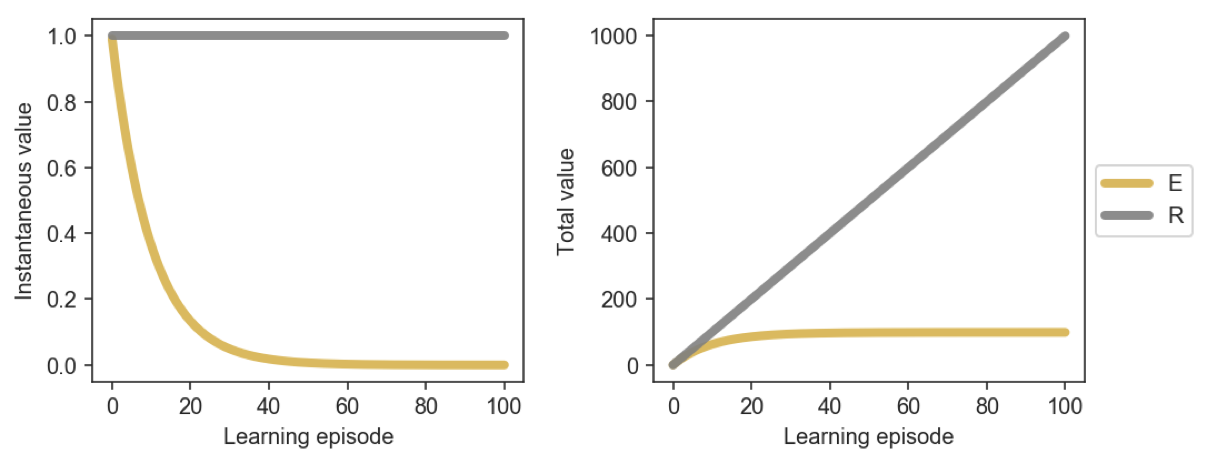
\includegraphics[scale=0.2]{images/E_time.png}
    \caption{Reward and information value.}
\end{figure}
\end{frame}

\begin{frame}[fragile]{Progress.}
\begin{enumerate}
\item Information is fundamental
\item An axiomatic definition for information value, $E$
\begin{itemize}
\item A minimal memory
\item A minimal distance
\item Value is the total distance the memory moves
\end{itemize}
\item Proven how to maximize $E$, optimally
\begin{itemize}
\item Every time step $t$ is greedy; always pick the biggest distance.
\end{itemize}
\end{enumerate}
\end{frame}

\begin{frame}[fragile]{\st{Goal.}}
\begin{itemize}
    \item Curiosity learning \textit{has} a clear and common objective:
    \begin{itemize}
        \item $ \max \sum_T E$
    \end{itemize}
\end{itemize}
\end{frame}

\begin{frame}[fragile]{The dilemma.}
    \begin{quote}
        Should I exploit an available reward, or explore to try find more rewards? 
    \end{quote}
\end{frame}

\begin{frame}[fragile]{The dilemma.}
\begin{itemize}
    \item Reward is fundamentally valuable
    \item Information is fundamentally valuable
\end{itemize}
\end{frame}

\begin{frame}[fragile]{The dilemma.}
\begin{itemize}
    \item Reward is fundamentally valuable
    \item Information is fundamentally valuable
    \item Reward $\Leftrightarrow$ Information?
\end{itemize}
\end{frame}

% ---------
\begin{frame}[fragile]{Information is not a reward?}
\begin{itemize}
    \item Rewards are a conserved resource.
    \item Information is not.
\end{itemize}
\end{frame}

\begin{frame}[fragile]{Information is not a reward?}
\begin{itemize}
    \item Reward value is fixed(-ish).
    \item Information value is \textit{never} fixed when learning.
\end{itemize}
\end{frame}

\begin{frame}[fragile]{Big conjecture \#3.}
\begin{center}
    Information is not a reward.
\end{center}
\end{frame}

\begin{frame}[fragile]{Information is not a reward.}
\begin{columns}
\column{0.5\textwidth}
\textit{No:}
\begin{itemize}
    \item $R + E$
    \item $R + \beta I$
    \item $R + novelty$
\end{itemize}

\column{0.5\textwidth}
\begin{figure}
    \centering
    
\includegraphics[scale=0.4]{images/cake_book.png}
    \caption{}
\end{figure}
\end{columns}
\end{frame}

\begin{frame}[fragile]{Now we have two problems....}
\textit{Learn:}
\begin{enumerate}
    \item An action policy $\pi_R$ to $\max \sum_T R$
    \item An action policy $\pi_E$ to $\max \sum_T E$
\end{enumerate}
\end{frame}

\begin{frame}[fragile]{Dual value learning}
\textit{Solution:}
\begin{equation*}
    \label{eq:pipi} 
	\begin{split}
		\pi^{\pi} = 
		\begin{cases}
			\pi^*_E & : E - \eta > R \\
			\pi_R & : E - \eta \le R \\
		\end{cases}
		\\
		\text{subject to the constraints}\\
		R \in \{0, 1\} \\
		p(\mathbb E[R]) < 1 \\
		E - \eta \geq 0 \\
		\text{choose}\ E_0 > 0
	\end{split}
\end{equation*}
\begin{itemize}
\item (Proof by induction; it's a classic scheduling problem)
\end{itemize}
\end{frame}

\begin{frame}[fragile]{Optimality of $\pi^\pi$.}
\textit{Search}:
\begin{itemize}
\item \textit{If} M is complete in $S$, 
\item \textit{then} $S$ is searched completely and exhaustively
\end{itemize}
\end{frame}

\begin{frame}[fragile]{Optimality of $\pi^\pi$.}
\textit{Reward}:
\begin{itemize}
    \item \textit{If} $\pi^*_R$ and $M \leftarrow R$,
    \item \textit{then} $\max \sum_T R$ (or $\max \sum_T \gamma^t R$)
\end{itemize}
\end{frame}

\begin{frame}[fragile]{Optimality of $\pi^\pi$.}
\textit{No regret}:
\begin{itemize}
\item $G = 0$ for all $a \in A$ and $s \in S$
\item (Every choice is greedy in $\pi^{\pi}$)
\end{itemize}
\end{frame}

\begin{frame}[fragile]{Progress.}
\begin{itemize}
\item A no regret way to solve exploration-exploitation problems
\item Learns a/the necessary world model along the way
\begin{itemize}
    \item (Works for \textit{nearly} any world model)
\end{itemize}
\item Straight forward to ensure the best reward policy is found
\begin{itemize}
    \item (Works for \textit{nearly} on reinforcement learning rule)
    \item (...Just pick a \textit{good one})
\end{itemize}
\end{itemize}
\end{frame}

\begin{frame}[fragile]{In practice.}
\begin{itemize}
    \item \alert{Theoretical promises often fail in practice.}
    \item (But initial results look promising.)
\end{itemize}
\end{frame}

\begin{frame}[fragile]{$n$-armed bandits.}
\begin{figure}
    \centering
    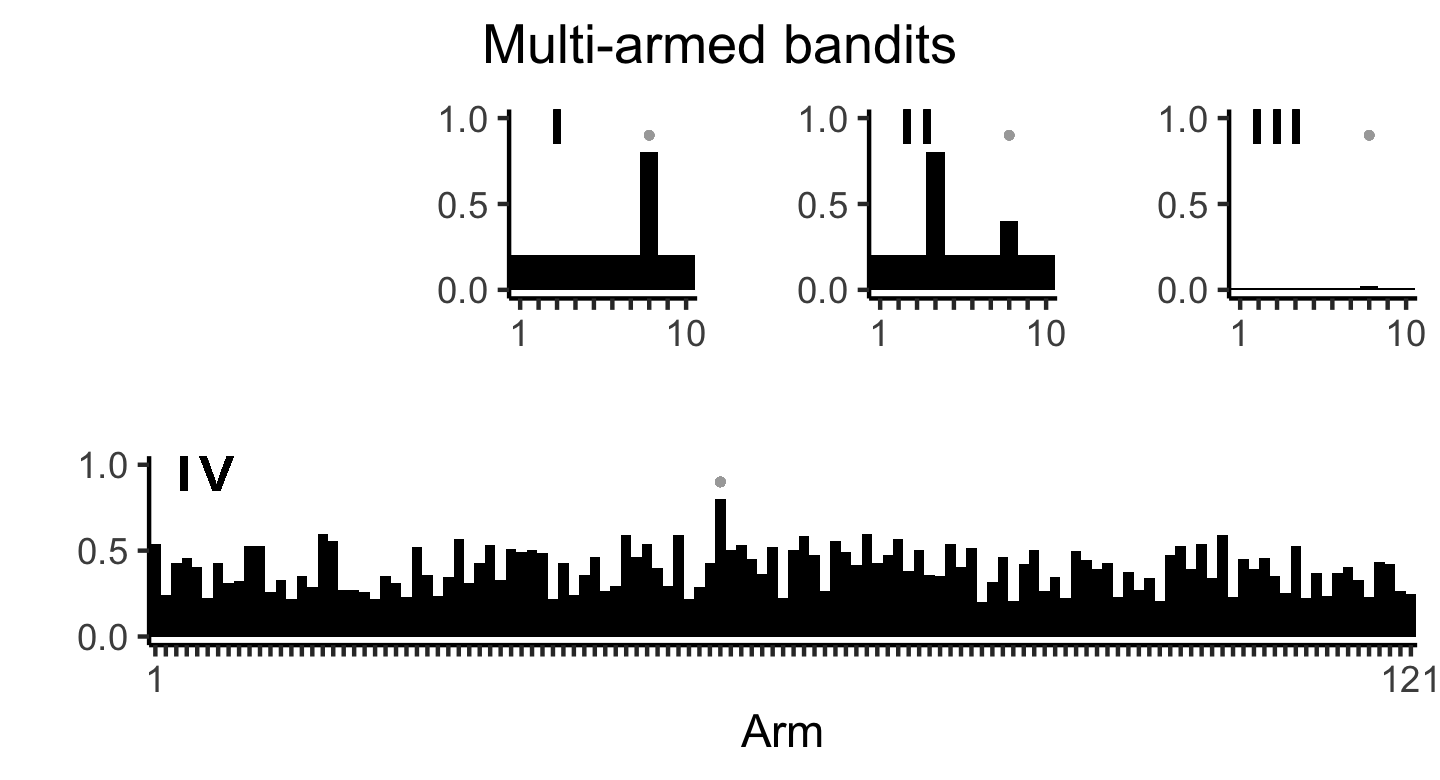
\includegraphics[scale=0.2]{images/fig2.png}
    \caption{}
\end{figure}
\end{frame}

\begin{frame}[fragile]{$n$-armed bandits.}
\begin{figure}
    \centering
    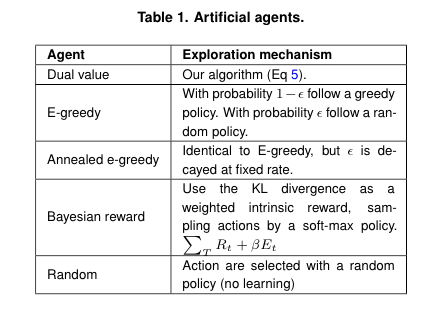
\includegraphics[scale=0.8]{images/agents.png}
    \caption{}
\end{figure}
\end{frame}

\begin{frame}[fragile]{$n$-armed bandits.}
\begin{figure}
    \centering
    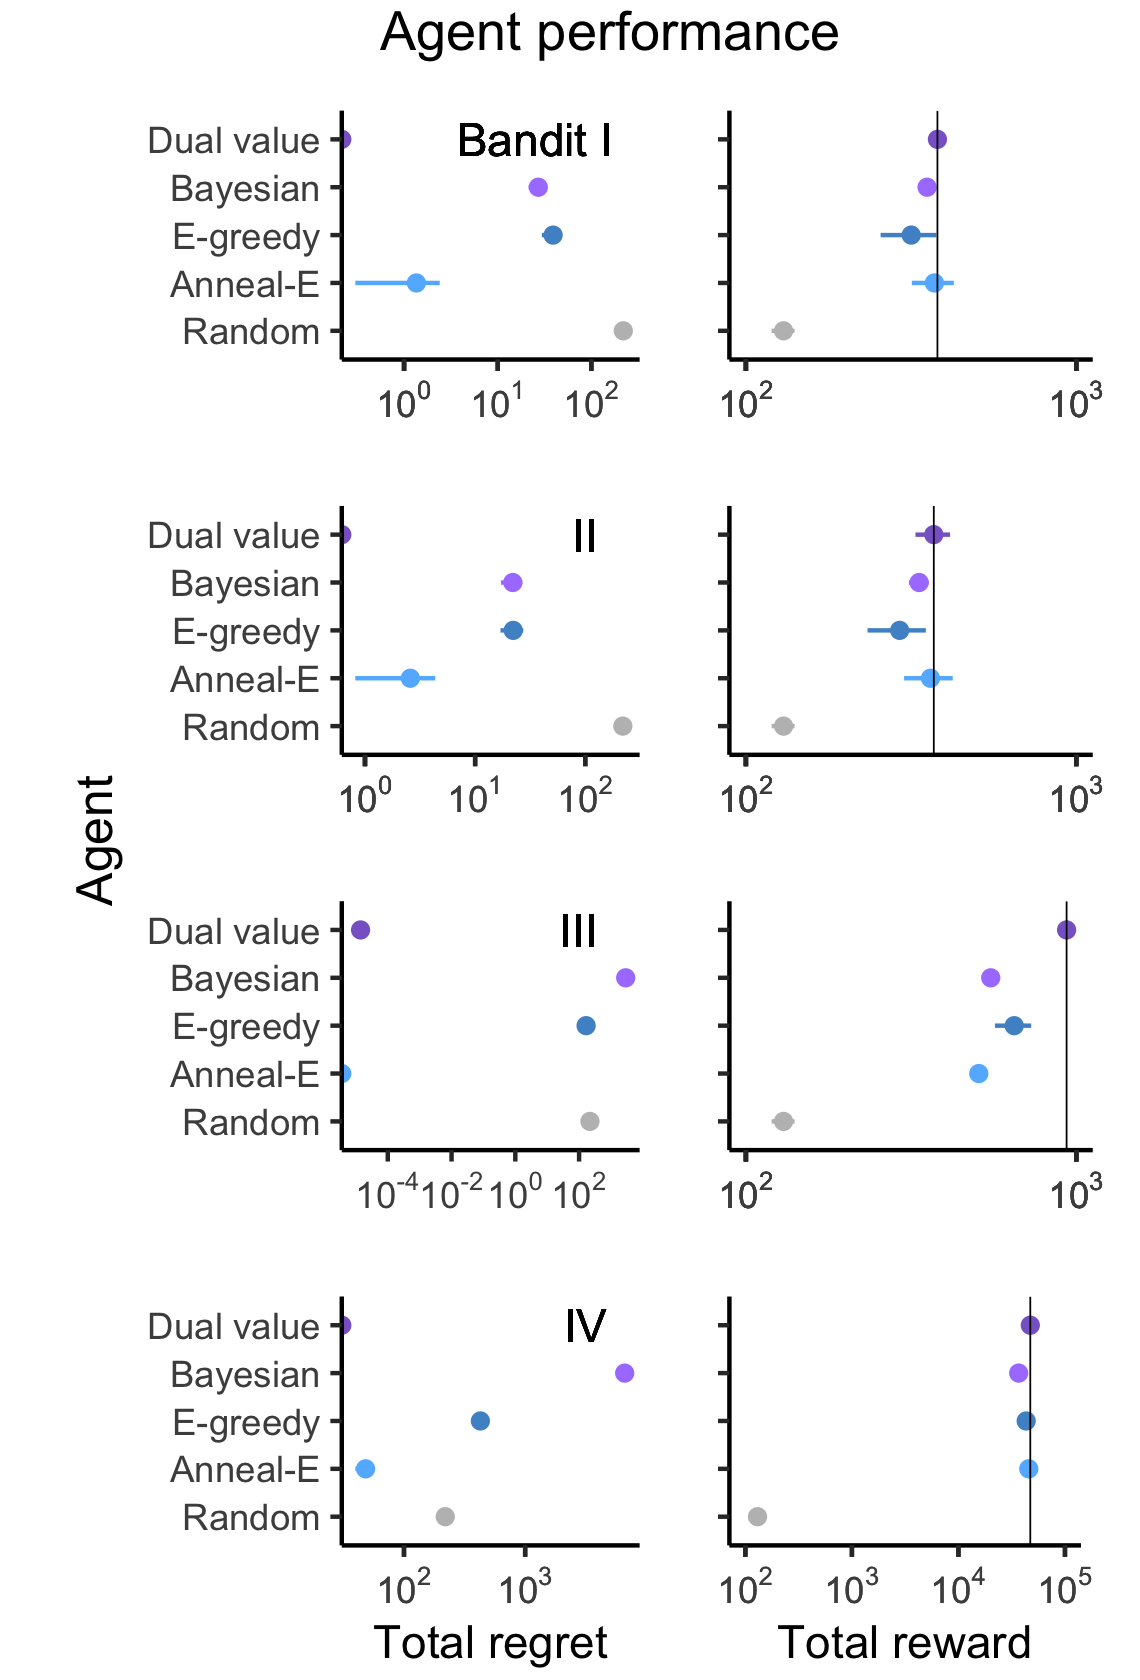
\includegraphics[scale=0.125]{images/fig3.png}
    \caption{}
\end{figure}
\end{frame}

\begin{frame}[fragile]{Do humans value information equally?}
\begin{figure}
    \centering
    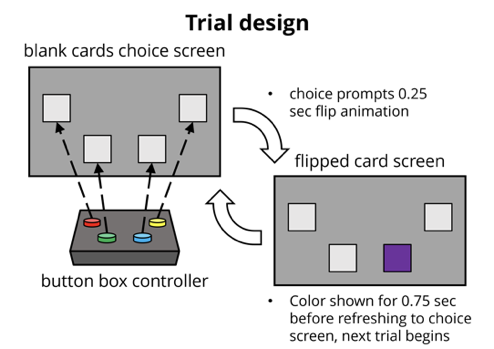
\includegraphics[scale=0.4]{images/bitjoy.png}
    \caption{The \textit{bitjoy} bandit task.}
\end{figure}
\end{frame}

\begin{frame}[fragile]{Bitjoy.}
\begin{figure}
    \centering
    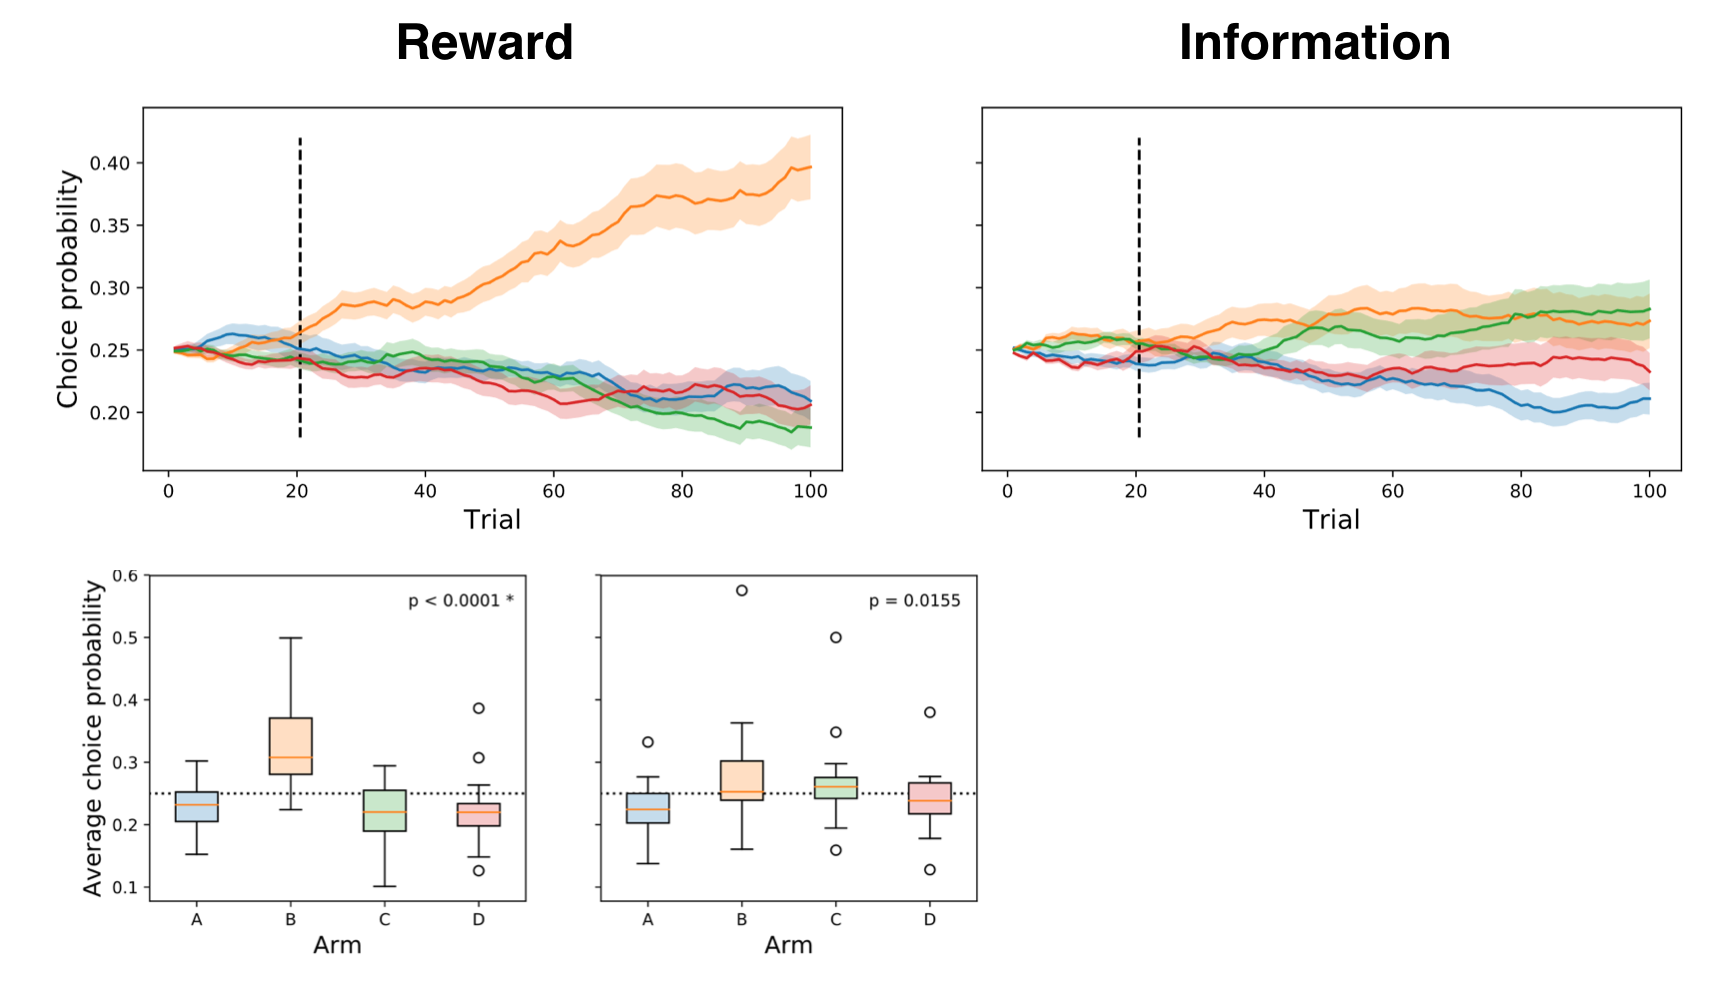
\includegraphics[scale=0.3]{images/bitjoy_main_results.png}
    \caption{Human behavioral performance ($n=24$).}
\end{figure}
\end{frame}

\begin{frame}[fragile]{Conclusions.}
\begin{itemize}
    \item Don't explore to get rewards.
    \item Explore to learn.
    \item You'll have no regrets, and the reward will come.
\end{itemize}
% TODO right bee here in other col
\end{frame}

\begin{frame}[fragile]{Future work.}
\textit{Explore deterministic (optimal) exploration in:}
\begin{itemize}
    \item Artificial intelligence
    \item Animal behavior
\end{itemize}
\end{frame}

\begin{frame}[fragile]{Open science.}
\begin{itemize}
\item[Paper] \url{biorxiv.org/content/10.1101/671362}
\item[Code] \url{github.com/CoAxLab/infomercial}
\item[Talk] \url{github.com/parenthetical-e/dilemma-talk-irvine-2019}
\item[] 
\item[] \alert{Thank you!}
\end{itemize}
\end{frame}

\begin{frame}[fragile]{Hire me!}
\begin{figure}
    \centering
    
\includegraphics[scale=0.15]{images/bunny_ears_me.jpg}
    \caption{\url{robotpuggle.com}}
\end{figure}
\end{frame}

% ---------------------------------------------------------
\begin{frame}[allowframebreaks]{References}
  \bibliography{library}
  \footnotesize{\bibliographystyle{abbrv}}
\end{frame}

% ---------------------------------------------------------
\end{document}
